\section{Internal Communication}
\label{design:internalcomm}

We also have to consider internal communication between the bootware core and plugins, and possibly also in between plugins.
Ideally, every plugin will be able to react to events from the bootware.
These event could be triggered by the bootware core or by any plugin, but plugins should be completely independent from each other.
Since a plugin doesn't know about other plugins, it can't listen for events at other plugins directly.
The only known constant to a plugin is the bootware core.
Therefore we need a communication mechanism which allows for loosely coupled communication between the bootware core and the plugins, where plugins can register their interest for certain events with the core and also publish their own events to the core for other plugins to consume.
This essentially describes the publish-subscribe pattern~\autocite{pubsub}.

\subsection{PubSub}

The \nom{publish-subscribe pattern}{PubSub} is a messaging pattern that consists of three types of participant: A event bus (or message broker), publishers, and subscribers.
The event bus sits at the center of the communication.
He receives messages from publishers and distributes them to all subscribers that have voiced their interest in messages of a certain type by subscribing at the event bus~\autocite{pubsub}.

Using this pattern in our bootware component, we would create an event bus at the bootware core and plugins, as well as other parts of the core, could subscribe at this event bus and also publish messages through this event bus.

\begin{figure}[!htbp]
	\centering
	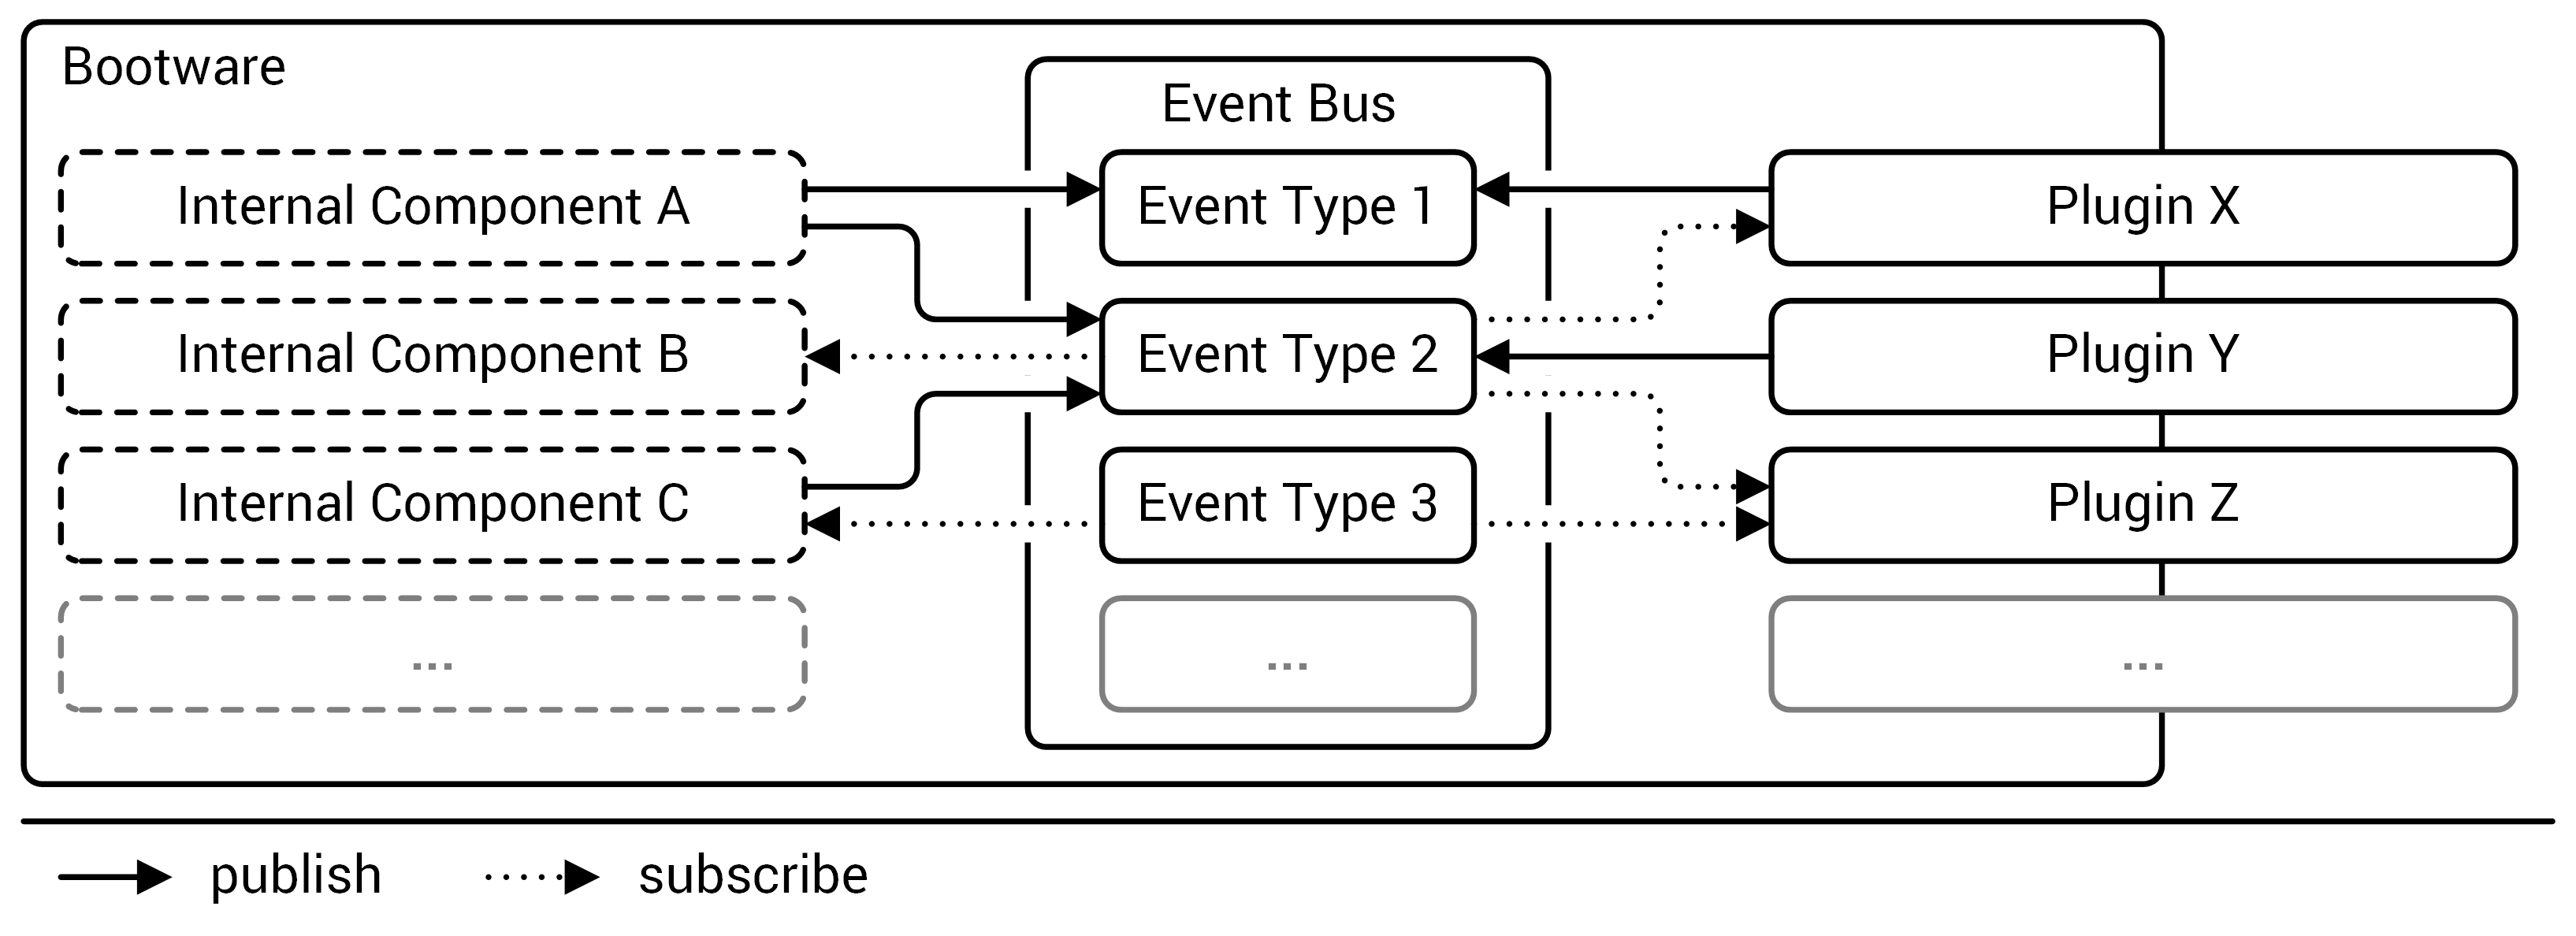
\includegraphics[resolution=600]{design/assets/pubsub}
	\caption{Bootware internal communication with PubSub pattern.}
	\label{image:pubsub}
\end{figure}

\subsection{Event Types}

When using PubSub and events to communicate, its usually a good idea to not only use one type of event, but many different types.
As an example, it would make sense to not only use one event type to communicate the bootstrapping process, but to divide those events into distinct groups based on their importance or general contents.
In this case, we could use four different event types: Info events, success events, warning events, and error events,
Info events would be used for general, non-critical information.
Success events would be used each time a process step was completed successfully.
Warning event would be used when something went slightly wrong but the overall process can still continue.
Error event would be used if something really went wrong and the bootstrapping process will be aborted as a result of that.

Using different kinds of event allows us to react differently based on the type of the event.
But what if we want to react to each event type in the same way, for example for logging purposes?
Now, many different event types complicate things more.
This is where event hierarchies become useful.
In an event hierarchy, those four events mentioned before would all be derived from a more generic parent event.
This makes event handling much easier, since we can now just react to the parent event if we don't need to distinguish between different event types for a particular task.

As we can see, we might benefit from a well thought-out event hierarchy.

\textcolor{red}{MORE}
